% Boundary refinement viewed as a graph cut on the key similarity matrix.
% A small toy example: 8 tokens, surprise picks position 4 as a candidate
% boundary; refinement evaluates positions 3 and 5 too and picks the one
% whose induced two-community split scores best.

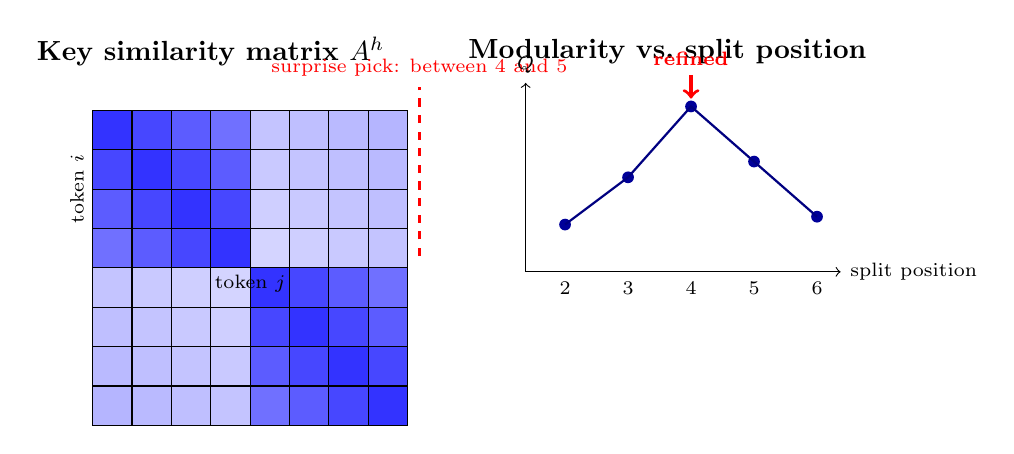
\begin{tikzpicture}[
  font=\footnotesize,
  cell/.style={draw, rectangle, minimum width=0.5cm, minimum height=0.5cm, inner sep=0pt},
  node distance=0.5cm,
]

% --- Left panel: similarity matrix as a heatmap ---
\begin{scope}[xshift=0cm, yshift=0cm]
  \node[font=\bfseries] at (2.0, 3.0) {Key similarity matrix $A^h$};

  % Generate an 8x8 grid with two block-diagonal communities at positions 1-3 and 5-8.
  % Color intensity ~ similarity. Within-cluster is darker.
  \foreach \i in {1,...,8} {
    \foreach \j in {1,...,8} {
      \pgfmathsetmacro{\val}{
        ifthenelse((\i<5 && \j<5) || (\i>4 && \j>4),
          80 - 8*abs(\i-\j),    % within-cluster
          15 + 2*abs(\i-\j))    % across-cluster
      }
      \pgfmathsetmacro{\colorval}{min(100, max(5, \val))}
      \node[cell, fill=blue!\colorval!white]
        at ({\j*0.5 + 0.25}, {2.5 - \i*0.5}) {};
    }
  }

  % Candidate boundary line at position 4-to-5 (surprise pick).
  \draw[red, very thick, dashed] (4.65, 0.4) -- (4.65, 2.55) node[above, font=\scriptsize] {surprise pick: between 4 and 5};

  % Axis labels.
  \node[font=\scriptsize] at (2.5, 0.05) {token $j$};
  \node[font=\scriptsize, rotate=90] at (0.3, 1.25) {token $i$};
\end{scope}

% --- Right panel: modularity score at each candidate split position ---
\begin{scope}[xshift=6.0cm, yshift=0.2cm]
  \node[font=\bfseries] at (1.8, 2.8) {Modularity vs.\ split position};

  % Axes
  \draw[->] (0, 0) -- (4.0, 0) node[right, font=\scriptsize] {split position};
  \draw[->] (0, 0) -- (0, 2.4) node[above, font=\scriptsize] {$Q$};

  % Data points: a peak at position 4 (correct boundary), lower at 3 and 5.
  \foreach \x/\y/\lbl in {0.5/0.6/2, 1.3/1.2/3, 2.1/2.1/4, 2.9/1.4/5, 3.7/0.7/6} {
    \node[circle, fill=blue!60!black, inner sep=1.5pt] at (\x, \y) {};
    \node[below, font=\scriptsize] at (\x, 0) {\lbl};
  }

  % Connect them.
  \draw[blue!50!black, thick]
    (0.5, 0.6) -- (1.3, 1.2) -- (2.1, 2.1) -- (2.9, 1.4) -- (3.7, 0.7);

  % Mark the chosen split with a red arrow.
  \draw[red, very thick, ->] (2.1, 2.5) -- (2.1, 2.2);
  \node[red, font=\scriptsize\bfseries, above] at (2.1, 2.5) {refined};
\end{scope}

\end{tikzpicture}
